\scanpage{327}
% archive sheet number: 328

$X$ courbe alg. / $\mathbb C$ proj. non sing conn genre $g\geq2$

Il y a sur $X$ un \deleted{fibré principal}\inserted{torseur} canonique
$P$ de grpe $\operatorname{GP}(1)_{\mathbb C}=G'_{\mathbb C}$ à connexion intégrable
(compatible \unsure{à|sa} structure de torseur), obtenu
ainsi : $\forall x\in X\longmapsto\widetilde X(x)$ rev. universel de $X$ en $x$
$\widetilde X(x)$ \deleted{$\unsure{\longleftrightarrow|\simeq|\Longleftrightarrow}$} \deleted{\unsure{demi-plan disque}}\inserted{demi-plan de} Poincaré $D$

\unsure{ens|un} des iso $\operatorname{Iso}((D,0),(\widetilde X(x),\tilde x))$ est un torseur à droite
\margin{\unsure{Or|On}}
sur $\operatorname{Isot}(D,0)\simeq\deleted{\operatorname{GP}(1)_{\mathbb R}\unsure{\subset|\simeq}G'_{\mathbb C}}\inserted{S_{\mathbb R}}$, d'où par ext. un
torseur à droite sur $G'$, \deleted{un \unsure{candidat pour G}}\inserted{soit $P_x$}.

On sait que les $P_x$ $(x\in X(\mathbb C))$ sont les fibres
d'un fibré principal \deleted{\unsure{analytique plat}}\inserted{top.} strictement plat
(celui associé à $\pi_{\unsure{1|x}}\longrightarrow G'_{\mathbb R}\subset G'_{\mathbb C}$)

\figure{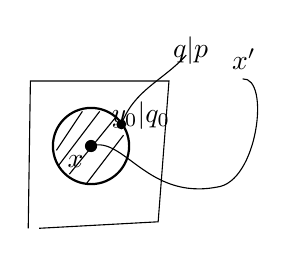
\begin{tikzpicture}[x=0.55cm,y=0.55cm]
\draw (0,0)--(0.05,3.4)--(3.25,3.4)--(3,0.15)--(0.25,0);
\draw[thick] (1.45,1.9) circle (0.88);
\draw (0.65,1.8)--(1.25,2.7) (0.7,1.45)--(1.65,2.7) (0.95,1.25)--(2.05,2.6) (1.35,1.04)--(2.2,2.15);
\fill (1.45,1.9) circle (2.2pt) (2.15,2.4) circle (1.8pt);
\node[below left] at (1.5,1.9) {$x$};
\draw (2.15,2.4).. controls (2.45,3.2) and (3.1,3.4)..(3.65,4.0);
\node at (3.75,4.1) {$\unsure{q|p}$};
\node at (2.6,2.6) {$\unsure{y_0|q_0}$};
\draw (1.45,1.9).. controls (2.2,2.15) and (2.75,0.65)..(4.35,0.95)
.. controls (5.3,1.05) and (5.6,3.5)..(4.95,3.45);
\node[above] at (4.98,3.45) {$x'$};
\end{tikzpicture}}

\uline{Th} $\forall x\in X$, $\exists$ une et une seule \deleted{\unsure{imm}}\inserted{imm.}
\unsure{ouverte|ouvert} analytique de $\widetilde X(x)$ dans
$T_x(X)$ dont a) l'image est un disque
b) l'application tangente en $\tilde x$
est l'identité.

\[
\pi_1(X,x)\underset{\unsure{j|?}}{\subset}G'\hookrightarrow G'_{\mathbb C}
\qquad \unsure{\mathcal U}
\]

\[
\begin{pmatrix}a&b\\c&d\end{pmatrix}.z=
\qquad
\begin{matrix}a\unsure{{}^{\ast}}&b\\-b&a\end{matrix}
\]

\[
\deleted{\unsure{alg|\deg}}\ \underline{P(x,q)}
\qquad Q_{\mathbb R}\qquad\text{\textcircled{\ensuremath{P_{\mathbb R}}}}\qquad
P(x,\rho\unsure{q})=P(x,x)\mathbin{\wedge}_{\operatorname{int}(\rho)}G'_{\mathbb C}
\]
\[
\begin{aligned}
P(x,\rho q)&=P(x,q)\mathbin{\wedge}_{\operatorname{int}(\rho)}G_{\mathbb C}\\
\unsure{q(q)|\rho}&\in\unsure{S'|S^1}\subset G'\subset G'_{\mathbb C}\\
&\mathbb C^{\ast}\quad Q_{\mathbb C}
\end{aligned}
\]
\diagram{\begin{tikzcd}[ampersand replacement=\&,row sep=small]
S_{\mathbb R}\arrow[r,phantom,"\subset" description]\arrow[d,phantom,"\cap" description] \& G'_{\mathbb R}\arrow[d,phantom,"\cap" description] \& {}\\
S_{\mathbb C}\arrow[r,phantom,"\subset" description] \& G'_{\mathbb C} \& P_{\mathbb C}
\end{tikzcd}}

\diagram{\begin{tikzcd}[ampersand replacement=\&,row sep=small]
P(x,q)\arrow[d,"\unsure{2}"'] \& G'_{\mathbb C}\arrow[d,"{\operatorname{int}(\unsure{\theta|\rho})}"]\\
P(x,x') \& G'_{\mathbb C}
\end{tikzcd}}

\[
E\longrightarrow E\otimes\Omega
\]
\figure{
\begin{tikzpicture}[x=0.45cm,y=0.45cm]
\draw (0,0) ellipse (1.05 and 1.15);
\draw (-0.83,-0.35)--(0.12,0.94) (-0.58,-0.71)--(0.7,0.83)
(0.13,-0.55)--(0.56,0.09)--(0.28,-0.62)--(0.84,-0.07);
\fill (0.06,0.08) circle (2pt);\draw (0.06,0.94) circle (1.3pt);
\end{tikzpicture}}
\[
E\longrightarrow E\otimes\Omega
\]

\diagram{\begin{tikzcd}[ampersand replacement=\&,row sep=tiny]
\mathbb C^{\ast}=\operatorname{GL}(2,\mathbb R)\arrow[d]\\
\operatorname{GL}(2,\mathbb C)
\end{tikzcd}}

a) fibré inversible : $\underline{\Omega^{-1}}$\qquad
$\mathbb G_m\longrightarrow\operatorname{GP}_{\unsure{k|\mathbb C}}$

b) \deleted{fibré}\inserted{un} $\mathrm P(\Omega^{-1}+\Omega)$ avec
conn. intégrable

\[
\begin{pmatrix}\Omega&0\\\Omega^3&\Omega\end{pmatrix}
\]

\fbox{\parbox{0.65\linewidth}{Trouver une connexion intégrable
(alg) canonique sur
\[
\mathrm P(\Omega^{-1}+\Omega)=\overline{\mathrm V(\Omega^2)}
\]}}

\[
\begin{aligned}
\Omega^{-1}\oplus\Omega&\longrightarrow(\Omega^{-1}\oplus\Omega)\otimes\Omega\\
&=\Omega_X^0+\Omega^2.
\end{aligned}
\qquad (D,\omega)=(\unsure{d},\infty,\Delta)
\]
